\begin{frame}
  \frametitle{Clustering images}

  \begin{center}
    Clustering is an \textit{unsupervised} learning task by which we
    look for structure in the data, grouping similar examples together
    \vskip20pt
    \only<1>{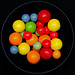
\includegraphics[height=0.25\textheight]{../../code/image_data/candy.jpg}}
    \only<2>{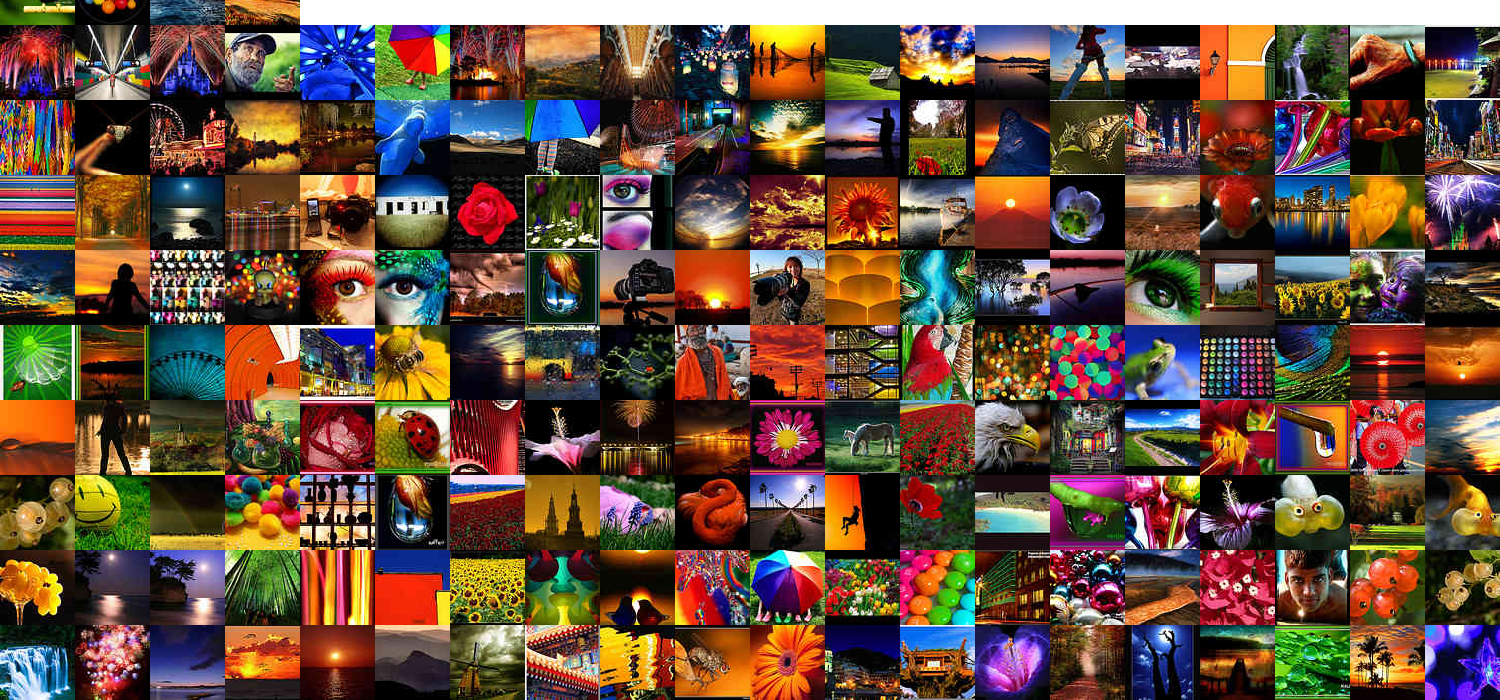
\includegraphics[height=0.25\textheight]{../../code/image_data/flickr_vivid_cluster_0}}
    \vskip20pt
    \only<1>{e.g., find groups of similar pixels within a single image}
    \only<2>{e.g., find groups of similar images across a collection of images}
  \end{center}

\end{frame}

\begin{frame}
  \frametitle{Clustering pixels}

  \begin{center}
  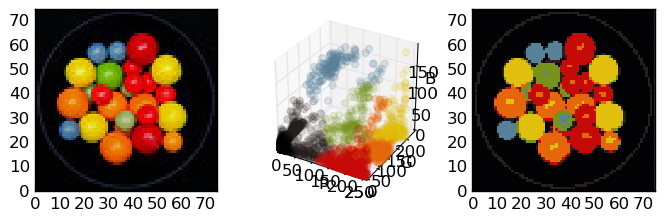
\includegraphics[width=\textwidth]{../../code/image_data/candy_clustered.png}
  \end{center}

\end{frame}


\begin{frame}
  \frametitle{Clustering images}

  \begin{center}
  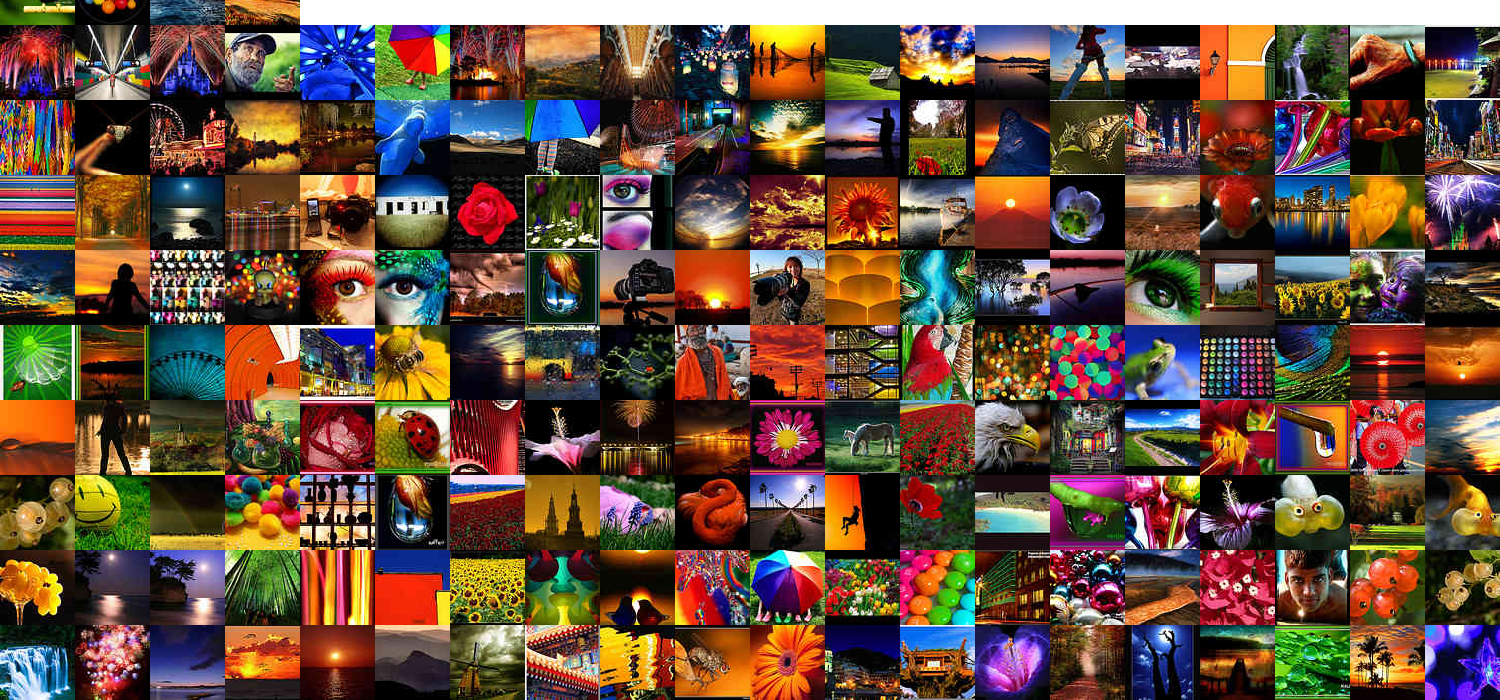
\includegraphics[width=\textwidth]{../../code/image_data/flickr_vivid_cluster_0.png}
  %\includegraphics[width=\textwidth]{flickr_vivid_clusters.pdf}
  \end{center}

\end{frame}
